
\chapter{序論}\label{chapter:序論}
第\ref{chapter:序論}章では,本研究の背景と先行研究,そして研究の目的を述べる.


\section{背景}

% 流れ
% 多脚ロボットの特徴と,不整地の移動に適していることを述べる
% 不整地の移動において,6脚であることによる利点を述べる
% 適応歩容の必要性を述べる
% 適応歩容の実現方法を述べる,そして,グラフ探索による手法を述べる

% 1.1.1 章
\subsection{多脚ロボットの対環境適応性能}
近年,人間に代わって作業を行う移動ロボットの導入が進められている.
Pudu社が開発したロボットのBellaBotが,レストランで配膳の作業を行う姿は一般に見ることができるようになった.
これらのロボットの多くはタイヤやクローラを用いての移動を行うが,
その他の移動様式として,脚を使用して移動を行うロボット(以下脚ロボット)が存在する.
脚ロボットは他の移動様式を用いて移動するロボットに比べて,
以下に示すような利点がある\cite{Locomotion_for_difficult_terrain}.

\begin{itemize}
  \item 障害物をまたいで移動できるため,対地適応性が高い
  \item 脚接地点を離散的に選択できるため,環境に与える影響が小さい
  \item スリップすることなく全方向に移動できる
\end{itemize}

障害物をまたいで移動できることにより,脚ロボットはタイヤでは移動できないような凹凸が激しい地形や,不連続な地形においても移動することが可能である.
また,砂利で舗装された道のような,クローラではスリップしてしまうような環境においても移動することが可能である.
この特徴を生かして,実際に図\ref{fig:nedo_spot}のようにBoston Dynamics Inc. によって開発された4足歩行ロボットのSpot\cite{Boston_Dynamics_Spot}を用いて,
林業を行う山間地で作業を行う実証実験が行われている\cite{NEDO}.
山間地は斜面である上に,伐根作業によって木の根が残っているため凹凸が激しく,タイヤやクローラでは移動が困難である.
しかし,脚ロボットであるSpotは障害物をまたいで移動することができるため,このような環境での作業に適しており,
人手不足の解消や,作業効率の向上が期待されている.

また,離散的に脚接地地点を選択できるため,タイヤやクローラによる移動と比較して環境に与える影響が小さい.
この特徴を生かしたロボットの実例として,韓国海洋科学技術院によって開発された6脚ロボットのCrabster\cite{J_Kim_Dexterous_Crabster}があげられる.
図\ref{fig:crabster}に示したCrabsterは,流れの早い海底での作業を想定して開発されており,
6本の脚による移動や,4本の脚を海底に接地させ,残りの2本の脚を用いて作業を行うことが可能である.
脚を用いた移動では海底の砂を大量に巻き上げることがないため\cite{J_Kim_Little_Crabster},カメラを用いた観察や,センサを用いた地形の計測に優れている.

以上より,脚ロボットは不整地での使用に適していると言える.

\begin{figure}[htbp]
  \begin{center}
    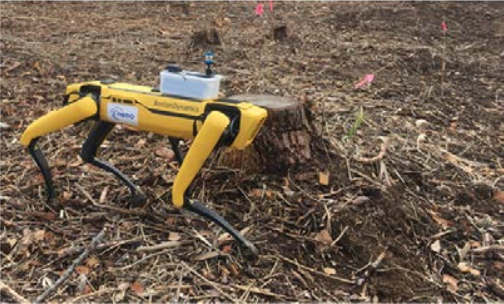
\includegraphics[width=100mm, clip]{figure/chapter1/NEDO.png}
   \caption{Demonstration Experiment with Spot\cite{NEDO}}
   \label{fig:nedo_spot}
  \end{center}
\end{figure}

\begin{figure}[htbp]
  \begin{center}
    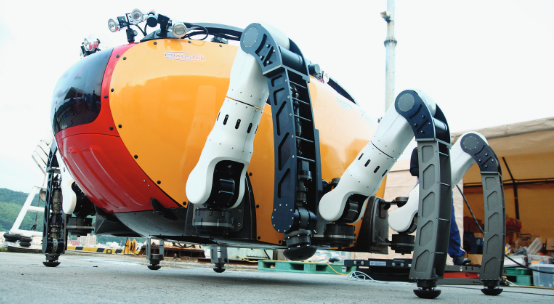
\includegraphics[width=100mm, clip]{figure/chapter1/crabster.png}
   \caption{Crabster\cite{J_Kim_Dexterous_Crabster}}
   \label{fig:crabster}
  \end{center}
\end{figure}

\subsubsection{多脚ロボットの静的安定性}
不整地を歩行する際は,ロボットが転倒することのないように常に静歩行を行うことが求められる.
静歩行とは重心の位置が常に接地した脚を頂点とする多角形内に存在するように歩行を行うことである.
2脚ロボットの場合,歩行の際には常に1脚が支持脚となり,もう1脚が遊脚となることから,
静歩行を行うためには重心の位置を脚先の足裏面積の内側に入るように制御する必要がある.
そのため,障害物をまたいで移動すること

ロボットの性能の指標として,歩行速度や消費エネルギーなどがあるが,不整地において用いることを考え,
静的安定余裕\cite{Hirose_Static_stability_criterion}(Stability Margin)を指標として分別することとする.
静的安定余裕とは,ロボットが静的に安定するために必要な脚位置と重心位置の関係を表す指標である.
支持脚を結んでできる多角形の重心が,支持脚の内部にある場合,ロボットは静的に安定する.
そのため,静的安定余裕では多角形の辺から重心までの距離を評価に用いる.
以上より,6

% 1.1.2 章
\subsection{固定歩容と自由歩容}
多脚ロボットが歩行を行う際には,脚を適切な順番で動かす必要がある.

歩容にはさまざまな種類があるが,大きく分別するとカムやリンクを用いて,
周期的に脚を動かす固定歩容と,非周期的に脚を動かす自由歩容がある.

\subsection{グラフ探索による自由歩容パターン生成手法}

本研究室においては,6脚ロボットの自由歩容パターン生成手法として,グラフ探索による由歩容パターン生成手法を提案してきた.
グラフ探索による自由歩容パターン生成手法は,脚位置や動作を離散化することで歩容をグラフに落としこみ,
そのグラフの探索によって数動作先までの歩容パターンの組み合わせを網羅的に調べ,最適な歩容パターンを選択する手法である.
この手法の特徴として,数動作先までを考慮して歩容パターンを生成するため,デッドロックに陥りにくいという点や,
効率的な歩容パターンを生成することができるという点が挙げられる.
グラフ探索による自由歩容パターン生成手法は4脚ロボットにおいて行われていたが\cite{Prabir_Graph_search},6脚ロボットにおいては行われていなかった.
これは,脚の本数が増えることで脚の動かし方の組み合わせが増えるため,実時間内の計算が困難になるためである.

そこで本研究室では,グラフ探索による自由歩容パターン生成手法を6脚ロボットに適用するため,
離散化された脚位置の組み合わせを利用してグラフの階層構造化を行った.
また,自由歩容パターン生成による接地地点の計算と脚軌道の生成を分離した.
これらによって,グラフ探索による自由歩容パターン生成手法を6脚ロボットに適用することが可能になった.

本研究室では,ロボットを動作させる地形やロボットの動作によって段階的に開発を行っており,
これまでに2次元空間において,直進動作\cite{Oki_Graph_search},目的姿勢での停止\cite{Nakaoka_Graph_search},
旋回動作\cite{Shina_Graph_search}を行うための歩容パターン生成手法の実装に成功した.
また3次元空間においても,離散化された脚位置の3次元空間への拡張\cite{Miura_Graph_search}を行うことで,
直進動作\cite{Hato_Graph_search}を行うための歩容パターン生成手法の実装に成功した.

\section{本研究の目的}
これまでの研究によって,3次元の不整地において,重心高さを変更しつつ,
自由歩容パターン生成を行うことが可能となった.
しかし低頻度ではあるが,グラフ探索に成功したとしても脚軌道が生成できず,その歩容パターン通りに歩行することできなくなり,
動作を停止してしまう問題が生じてしまった.

そこで本論文では,常に脚軌道生成に成功するような歩容パターン生成手法を提案し,
脚軌道生成の失敗による動作停止を防ぐことを目的とする.

\section{本論文の構成}
本論文は,全6章から構成される.

第2章「歩容パターンの再評価手法の提案」では,常に脚軌道生成が可能になる手法として,
歩容パターンの再評価手法を提案し,その機能を述べる.

第3章「歩容パターンの再評価手法の実装」では,提案したプログラムの実装方法を述べる.

第4章「再評価手法の有効性の確認のための歩行シミュレーション」では,
提案手法を用いたシミュレーション実験の結果を述べる.

第5章「常に脚軌道生成が可能な自由歩容パターン生成手法を用いた実機による歩行実験」
では,提案手法を用いた実機試験の結果を述べる.

第6章「結論」では本論文の結論と今後の課題を述べる.
